\chapter{Einführung}
\label{Einfuehrung}




\section{Nutzen und Erwartungen}
\label{Nutzen}

Lineare Baumstrukturen entstehen oft durch lineare Blockabhängigkeiten. Diese Abhängigkeiten sind jedoch oft nicht zwingend linear, sonder werden der Einfachheit halber vom Compiler so dargestellt. Beispiele hierfür finden sich oft in verschachtelten Strukturen von algebraischen Relationen. \\
Die folgende Rechnung \ref{eq:beispiel-addition} wird oft mit einem rechts- oder links-assoziativen Abhängigkeitsgraph abgebildet. Dies führt dazu, dass in Mehrkernsystem die einzelnen Operationen nicht parallel durchgeführt werden können.

\begin{equation} \label{eq:beispiel-addition}
a + b + c + d + e + f + g + h
\end{equation}

In einer links-assoziativen Baumstruktur (siehe Abbildung \ref{fig:links-assoziativer-baum}) ist ein linearer Programmfluss vorgegeben. Jeder Schritt baut hierbei auf die vorherige Operation auf. In Tabelle \ref{tab:links-assoziativer-baum} sind die Befehle aufgelistet, welche aus dem links-assoziativen Baum in Abbildung \ref{fig:links-assoziativer-baum} folgen. Die Befehle sollen hierbei für einem 2-Kern-System optimiert werden. Die Bezeichner \textit{t1} bis \textit{t7} stehen dabei für die einzelnen Teilbäume, beziehungsweise ihre Zwischenergebnisse. Wie zu sehen werden die Befehle nur auf einen Kern ausgeführt. Der andere Kern kann nicht agieren, da ihm immer eine Abhängigkeit zum Folgebefehl fehlt.\\

Wünschenswert wäre an dieser Stelle jedoch ein Befehlssatz, welcher auf Mehrkernsystemen (zum Teil) parallel ausgeführt werden kann. Dadurch könnten Prozessortakte und somit die Laufzeit des kompilierten Programmes eingespart werden.\\
Das Verfahren des Tree-Height-Balancing soll hierbei angewendet werden, um die links- oder rechts-assoziativen Bäume auszubalancieren. Sofern die Kinder eines Baumes nicht untereinander Abhängigkeiten aufweisen, können diese parallel vom Prozessor bearbeitet werden. Die führt zur Ausführung vom mehreren Befehlen innerhalb eines Taktes in Mehrkernsystemen.


\begin{figure}
	\begin{center}
	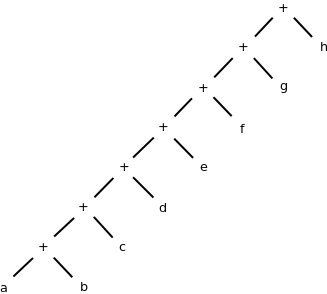
\includegraphics[width=0.5\textwidth]{images/links_assoziativer_baum}\\
	\end{center}
	\caption{Links-assoziativer Baum}
	\label{fig:links-assoziativer-baum}
\end{figure}

\begin{table}
	\begin{center}
			\begin{tabular}{|c|c|c|}
				\hline  & Kern 1 & Kern 2 \\ 
				\hline 1 & $ t1 \leftarrow a + b $& - \\ 
				\hline 2 & $ t2 \leftarrow t1 + c $& - \\ 
				\hline 3 & $ t3 \leftarrow t2 + d $& - \\ 
				\hline 4 & $ t4 \leftarrow t3 + e $& - \\ 
				\hline 5 & $ t5 \leftarrow t4 + f $& - \\ 
				\hline 6 & $ t6 \leftarrow t5 + g $& - \\ 
				\hline 7 & $ t7 \leftarrow t6 + h $& - \\ 
				\hline 
			\end{tabular}
	\end{center}
	\caption{Befehle für links-assoziativen Baum}
	\label{tab:links-assoziativer-baum}
\end{table}

